\documentclass[12pt]{article}
\usepackage{graphicx}
\usepackage{hyperref}
\usepackage{setspace}
\usepackage{caption}
\usepackage{geometry}
\usepackage{float}
\usepackage{booktabs}
\geometry{margin=1in}
\setstretch{1.25}

\title{What If St. Paul Made Vacant Landowners Pay for the Budget Shortfall?}
\author{Matthew Hockert}
\date{\today}

\begin{document}
\maketitle

A while back I was reading the Axios Twin Cities newsletter and its reporting on the proposed budget from St. Paul Mayor Melvin Carter that he argues avoids layoffs of city workers but raises the property tax levy by 5.3\%. The plan comes as the city faces a \$23 million deficit heading into 2026.  

Property taxes make up almost half (46\%) of St. Paul's \href{https://www.stpaul.gov/sites/default/files/2024-02/2024%20City%20of%20Saint%20Paul%20Adopted%20Operating%20Budget.pdf}{general fund} in 2024. Given it's a significant source of funding and itself a key instrument in keeping the lights on the city is limited in how it can make adjustments. The city is stuck with a blunt tool whereby it must levy higher taxes to make up for the shortfall. The bluntness of this tool is much worse when you think about how St. Paul can only raise property taxes uniformly across property classes, which means everyone pays more, regardless of whether their property is sitting vacant or fully developed. Cities like St. Paul don’t have the authority to vary tax rates based on land use, those classifications are set by the state legislature.  

But St. Paul can adjust certain fees, including the one for vacant buildings, which got me thinking:  

\begin{quote}
What if, instead of raising everyone’s property taxes, St. Paul raised the fees on vacant lots to make up the shortfall?
\end{quote}

\section*{Why It’s Interesting}

This post is purely a hypothetical scenario and an exercise for me as an economist. It is not meant as a formal fiscal policy proposal, but actually to highlight how fee structures, rules on local governance, and how changes in these two can influence behavior. Under Minnesota law the distinction between taxes and fees is significant and ultimately shapes who bears the costs of fiscal shortfalls.

As highlighted above, property taxes are a significant source of general fund revenue and can be used broadly to support the operations of a city. By contrast, fees are much more constrained under the law: they must be tied to the cost of providing a specific service or regulating an activity. For example, a sewer fee can only fund wastewater infrastructure, and a vacant building registration fee can only support code enforcement or maintenance associated with those properties.

Therefore, St. Paul could not legally use higher vacant property fees to make up for the property tax levy increase without legislative action. However, this blog is for fun but may also serve to show how fees can alter the incentives on underutilized land. This approach could, in theory, encourage redevelopment and reduce the number of idle parcels, strengthening the long-run tax base while minimizing impacts on homeowners. (Yes this is essentially a Land Value Tax (LVT) targeting only vacant parcels).


\section*{Methods}

All data and analysis were performed in R, and you can find the code in my \href{https://github.com/MatthewHockert/vacant_land_fees_st_paul_blog}{GitHub repository}. The workflow consisted of two main stages:

\begin{enumerate}

    \item Vacancy classification. Parcels were identified as vacant if their \texttt{DWELL\_TYPE} field included the terms ``VACANT'' or ``UNIMPROVED,'' and both \texttt{EMV\_BLDG == 0} and \texttt{NUM\_UNITS == 0}. A binary indicator variable, \texttt{vacant\_strict}, was assigned to flag these parcels. Parcels associated with redevelopment projects (e.g., ``FORD LOT'' or ``HIGHLAND BRIDGE ROWHOMES'') were excluded because, by 2025, many have been developed.

    \item Fiscal simulation. The city’s total levy (\texttt{city\_levy\_est}) was estimated from parcel tax capacity and an assumed city tax rate (\texttt{city\_rate = 0.497}). The city tax rate was derived by dividing the total levy by the city’s aggregate tax capacity, as documented \href{https://www.stpaul.gov/sites/default/files/2024-08/Major%20City%20General%20Fund%20Revenues%202025%20Proposed.pdf}{here}. A hypothetical shortfall of 5.3\% was then applied to this levy to represent the 2024 budget gap. \\

    Rather than simply dividing \$23 million by the number of vacant parcels, I simulate the shortfall using parcel-level tax capacity data to anchor the results in reality. This approach allows me to place the 5.3\% shortfall into 2024 and estimate a levy, tax base, and the rate used to calculate parcel-level taxes. This I feel is a more robust and interpretable approach within the context of the city’s fiscal system.
\end{enumerate}

\section*{Vacant Building Regulations}

According to the City of St. Paul, property owners must register vacant or unoccupied buildings with the Department of Safety and Inspections. You can read the list of criteria \href{https://www.stpaul.gov/departments/safety-inspections/rent-buy-sell-property/vacant-buildings/vacant-building-program}{here}.

Under the Saint Paul Legislative Code, \href{https://library.municode.com/mn/st._paul/codes/code_of_ordinances?nodeId=PTIILECO_TITVIBUHO_CH43VABU_S43.03VABURE}{Section 43.02}, owners of registered vacant buildings are required to pay an annual registration fee. The fee is designed to recover the city’s administrative and enforcement costs associated with monitoring these properties. In this post, I am creating a hypothetical world where we can use these fees to offset the budgetary shortfall and not have to use the fees in the traditional way. The fee schedule is structured by category as follows:

\begin{itemize}
    \item Category I: \$2,705 per year.
    \item Category II: \$2,705 in the first year and \$5,410 per year thereafter.
    \item Category III: \$5,410 per year.
\end{itemize}

\section*{Crunching the Numbers}

Using St. Paul’s 2024 parcel data and given my methods above, I calculate that there is roughly 1,339 vacant parcels. I then categorize the other types of parcels and divide them by their acreage. From the table below vacant land pays the least per acre (\$4,012) and the least amount in general (\$439), highlighting its inefficiency. When land is used this way other classifications make up for their lack of taxes.

\begin{table}[h!]
\centering
\caption{Average Property Tax by Super Class (2024)}
\begin{tabular}{llrr}
\toprule
\textbf{Rank} & \textbf{Super Class} & \textbf{Avg. Tax per Acre (\$)} & \textbf{Avg. Tax per Parcel (\$)} \\
\midrule
1 & Commercial & 22{,}841 & 12{,}990 \\
2 & Multi-Family Residential & 17{,}899 & 5{,}598 \\
3 & Manufacturing / Industrial & 12{,}350 & 20{,}231 \\
4 & Single-Family Residential & 10{,}513 & 1{,}521 \\
5 & Other / Unknown & 7{,}008 & 2{,}997 \\
6 & Agricultural & 4{,}684 & 9{,}927 \\
7 & Vacant & 4{,}012 & 439 \\
\bottomrule
\end{tabular}
\parbox{\linewidth}{\raggedright\footnotesize Source: Author’s calculations using 2024 St. Paul parcel data.}
\end{table}


The figure below shows the location of these vacant parcels. Some vacant parcels are concentrated near I-94 and along the Green Line corridor, with additional clusters on the city’s east side and a scattered across other neighborhoods. These are valuable locations that could be used for many other opportunities.

\begin{figure}[H]
    \centering
    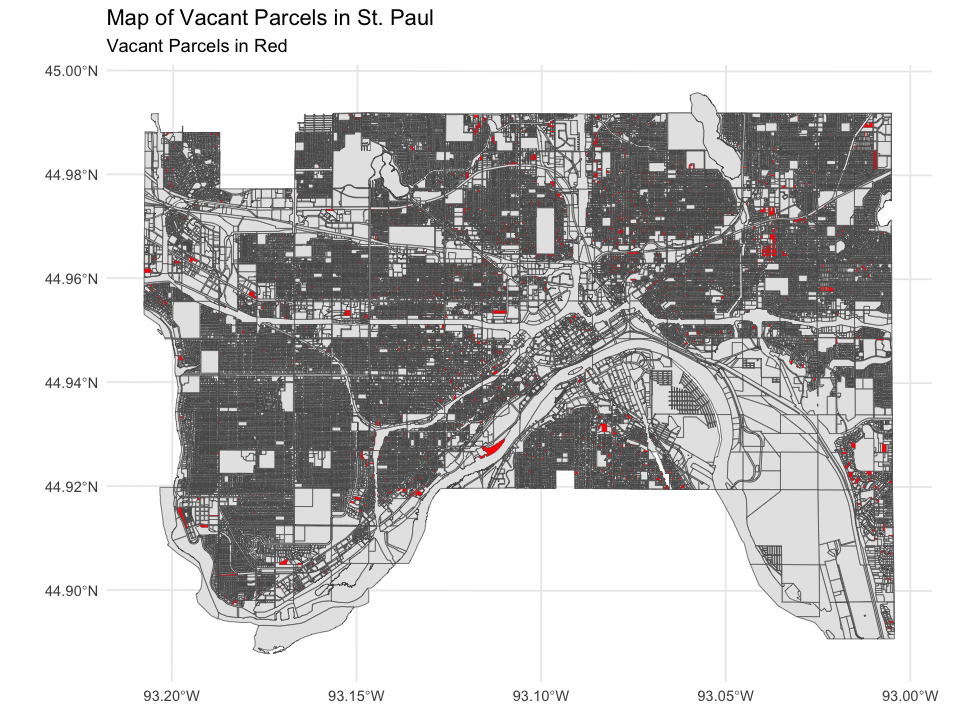
\includegraphics[width=0.9\linewidth]{Map of Vacant Parcels in St. Paul.png}
    \caption{St. Paul's vacant parcels mapped}
\end{figure}

Given that the current minimum vacant building fee is about \$2,705 per year. To cover the city’s shortfall without touching property taxes, those vacant parcels would need to carry the load through higher fees. Here’s what that looks like:

\begin{figure}[H]
    \centering
    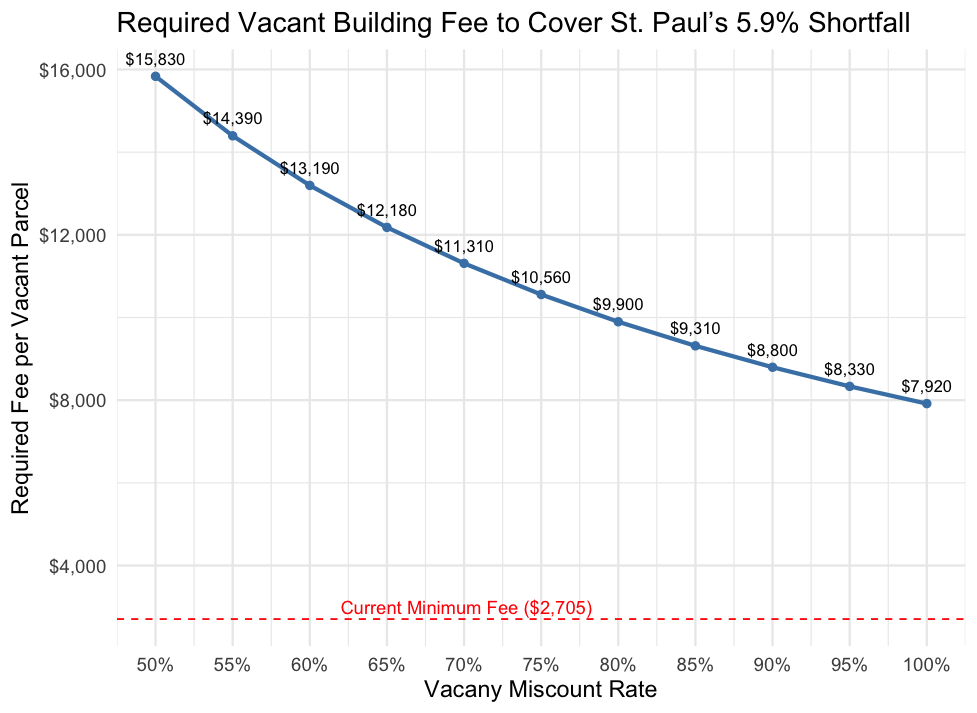
\includegraphics[width=0.9\linewidth]{st_paul_vacant_building_fee_graph.png}
    \caption{Required Vacant Building Fee to Cover St. Paul’s 5.9\% Shortfall}
\end{figure}

The chart shows how high the vacant lot fee would need to be, depending on how accurate my parcel count is.  

\begin{itemize}
    \item If I perfectly counted all 1,339 parcels (100\% on the right), each lot would need to pay about \$7,920 annually — nearly 3x the minimum fee.
    \item If I over counted by half (only about 700 real vacant parcels), the required fee would jump to nearly \$16,000 per parcel — almost 6x higher than the minimum.
    \item If we took the \$7,920 fee and added it on top of the \$439 average tax that vacant parcels are paying now, they would pay roughly \$8,359, which would only move the vacant parcels up three spots from the bottom in terms of average taxes from table 1.
\end{itemize}

\section*{Big Picture}

Taxes and inefficient land use affect all residents of the city. By taxing vacancy instead of productive land use, cities could encourage denser development and strengthen their long-term tax base, without overburdening homeowners, renters, and employers. This is in essence a targeted land value tax. However, in this hypothetical the most efficient parcels keep the their taxes the same rate as before, whereas in LVT the distribution would theoretically shift away from the most productive parcels to the least (vacant), further heightening the development pressure. This has a whole set of long run implications for the city's tax base depending on how quickly parcels are developed and what they ultimately become. One could argue that buying up vacant land and sitting on it is fair game and that this is just how the world is, but I think otherwise. We as a society chose to award the least productive through our policies and we all pay for it. For me it's better to imagine a different reality where these parcels become housing, parks, office space, restaurants, or whatever else. Putting the pressure on vacancy to become something more productive helps all residents by reducing the share of the city's tax burden. In a time where residents complain about higher property taxes and the how difficult it is for young people to stay in the city and start families, this hypothetical is an opportunity to open our minds to a better world where people can live here long term and not be priced out. For now, until cities can legally be more creative with their funding strategies, St. Paul’s budget reality means higher property taxes but it doesn't have to be. 

\end{document}